\documentclass{beamer}


\mode<presentation>
{
	\usetheme{Darmstadt}
	\setbeamercovered{transparent}
}

\setbeamertemplate{headline}{}

\usepackage[english]{babel}
\usepackage[utf8]{inputenc}
\usepackage{times}
\usepackage[T1]{fontenc}

\usepackage{calc}

\usepackage{tikz}

\usetikzlibrary{decorations.markings}

\tikzstyle{vertex}=[circle, draw, inner sep=0pt, minimum size=6pt]

\newcommand{\vertex}{\node[vertex]}

\newcounter{Angle}

\setbeamertemplate{bibliography item}[text]


\theoremstyle{definition}
\newtheorem{teor}{Theorem} 
\newtheorem{pro}{Proposition} 
\newtheorem{lema}{Lemma} 
\newtheorem{coro}{Corollary} 
\newtheorem{defn}{Definition}



\newcommand{\Li}{\mathcal{L}}
\newcommand{\C}{\mathcal{C}}
\newcommand{\D}{\mathcal{D}}
\newcommand{\W}{\mathcal{W}}
\newcommand{\R}{\mathcal{R}}
\newcommand{\M}{\mathcal{M}}
\newcommand{\N}{\mathcal{N}}
\newcommand{\V}{\mathcal{V}}
\newcommand{\E}{\mathcal{E}}
\newcommand{\J}{\mathcal{J}}
\newcommand{\Pa}{\mathcal{P}}
\newcommand{\I}{\mathcal{I}}
\newcommand{\up}{\upsilon} 
\newcommand{\Kmodel}{\bl\W,\R,\D,\I,\br}
\newcommand{\Fmodel}{\bl\W,\R,\D,\I,\E \br}
\newcommand{\p}{^{\prime}} 
\newcommand{\pp}{^{\prime\prime}}   
\newcommand{\nmodels}{\not\models}
\newcommand{\nao}{\neg}
\newcommand{\bige}{\bigwedge}
\newcommand{\e}{\wedge}
\newcommand{\see}{\longleftrightarrow}
\newcommand{\ou}{\vee}
\newcommand{\impli}{\rightarrow}
\newcommand{\bigou}{\bigvee}
\newcommand{\todo}{\forall} 
\newcommand{\ex}{\exists} 
\newcommand{\teo}{\vdash}
\newcommand{\vazio}{\emptyset}
\newcommand{\bl}{\langle}
\newcommand{\br}{\rangle}

%	\begin{frame}{Make Titles Informative.}
%		
%		You can create overlays\dots
%		\begin{itemize}
%			\item using the \texttt{pause} command:
%			\begin{itemize}
%				\item
%				First item.
%				\pause
%				\item    
%				Second item.
%			\end{itemize}
%			\item
%			using overlay specifications:
%			\begin{itemize}
%				\item<3->
%				First item.
%				\item<4->
%				Second item.
%			\end{itemize}
%			\item
%			using the general \texttt{uncover} command:
%			\begin{itemize}
%				\uncover<5->{\item
%					First item.}
%				\uncover<6->{\item
%					Second item.}
%			\end{itemize}
%		\end{itemize}
%	\end{frame}
%	


\setbeamertemplate{navigation symbols}{}%remove navigation symbols


\title[First-order justification logic JT45] 
{First-order justification logic JT45}


\author[F.Salvatore] 
{Felipe~Salvatore\inst{1}}

\institute[Universities of Somewhere and Elsewhere] 
{
	\inst{1}%
	graduate student in Philosophy\\
	University of São Paulo}


\date[CUNY 2015] 
{CUNY, Graduate Center, February 10, 2015}

\begin{document}
	
\begin{frame}
\titlepage 
\end{frame}


\begin{frame}
	\begin{itemize}
	\item[] {\color{blue}Motivations}
	\vspace{5mm}
	\item[] First-order modal logic
	\vspace{5mm}
	\item[] First-order justification logic
	\vspace{5mm}
	\item[] First-order JT45
	\vspace{5mm}
	\item[] Discussion: Realization
	\vspace{5mm}
	\item[] Discussion: Interpolation
	\end{itemize} 
\end{frame}

	

\begin{frame}{Motivations}

	
\begin{itemize}
\item Introduce justification terms into epistemic first-order logic.
\vspace{5mm}
\item Investigate the connection between justification logic and modal logic; in specific the role of the \textit{Interpolation Theorem}. It is well know that the Interpolation Theorem fails for first-order S5 (FOS5) \cite{Fine79}. And it is also well know that we can restore this theorem when we expand the expressive power of FOS5 either by adding propositional quantification \cite{Fitting02} or by adding the mechanisms of hybrid logic \cite{Areces01}.
\end{itemize}
\end{frame}

\begin{frame}
	\begin{itemize}
	\item[] Motivations
	\vspace{5mm}	
	\item[] {\color{blue}First-order modal logic}
	\vspace{5mm}
	\item[] First-order justification logic
	\vspace{5mm}
	\item[] First-order JT45
	\vspace{5mm}
	\item[] Discussion: Realization
	\vspace{5mm}
	\item[] Discussion: Interpolation
	\end{itemize} 
\end{frame}

\begin{frame}{First-order modal logic}
\qquad In few words, first-order modal logic is obtained when we add the modal operator $\Box$ to the language of first-order logic. Syntactically, this combination is simple, but to understand the meaning of the formulas we need to clarify some details. 

\qquad So, for example, the intended meaning of the formula \\
$$\ex x \Box (Q(x) \impli P(x))$$
is \\

\begin{center}
'there is an individual $x$ such that for every state, if $x$ has the property $Q$ then $x$ has the property $P$'
\end{center}
\end{frame}



\begin{frame}{First-order modal logic}
$M)$

	\[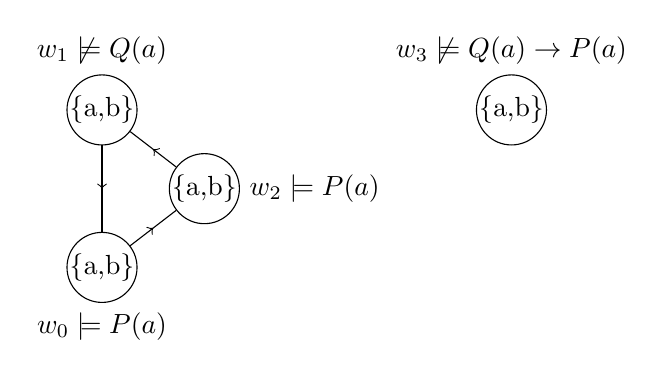
\begin{tikzpicture}[x=1.3cm, y=1cm,
	every edge/.style={
		draw,
		postaction={decorate,
			decoration={markings,mark=at position 0.5 with {\arrow{>}}}
		}
	}
	]
	\vertex (z) at (5, 2) [label=above:$w_{3} \nmodels Q(a) \impli P(a)$]{\{a,b\}};
	\vertex (v) at (1, 2) [label=above:$w_{1} \nmodels Q(a)$]{\{a,b\}};
	\vertex (x) at (2, 1) [label=right:$w_{2} \models P(a)$]{\{a,b\}};
	\vertex (y) at (1, 0) [label=below:$w_{0}\models P(a)$]{\{a,b\}};
	\path
	(v) edge node[right]{} (y)
	(x) edge node[right]{} (v)
	(y) edge node[pos=.4,right]{} (x)
	;
	\end{tikzpicture}\]	
	
	\qquad $M,w_{0} \models \ex x \Box (Q(x) \impli P(x))$
		
\end{frame}

\begin{frame}{Semantics} 

\begin{itemize}
\item A {\color{blue} S5 Skeleton} is a triple  $\bl \W, \R, \D \br$ where: $\W \ne \vazio$; $\R \subseteq \W \times \W$ such that $\R$ is an equivalence relation, and $\D \ne \vazio$.
	
\item A  {\color{blue} Kripke model} is a structure $M = \Kmodel$ where $\bl \W, \R, \D \br$ is an S5 skeleton; and:\\
 \vspace{5 mm}	

$\I$ is an \textit{interpretation function}, i.e.,  $\I$ is a function assigning to each $n$-ary relational symbol $Q$ and each $w \in \W$ an $n$-ary relation $\I(Q,w)$ on $\D$.

\end{itemize}
\end{frame}


\begin{frame}{Semantics} 
	Let $M = \Kmodel$ be a model, $\varphi$ a closed $\D$-formula and $w \in \W$. The notion \textit{$\varphi$ is true at world $w$ of $M$}, in symbols $M,w \models \varphi$, is defined as usual by induction on $\varphi$: 
	\begin{itemize} 
		\item $M,w \models Q(\vec{a})$ iff $\bl \vec{a}\br \in \I(Q,w)$. 
		\item $M,w \nmodels \bot$. 
		\item $M,w \models \psi \impli \theta$ iff $\M,w \nmodels \psi$ or $M,w \models \theta$.
		\item $M,w \models \todo x \psi(x)$ iff for every $a \in \D$, $M,w \models \psi(a)$.
		\item $M,w \models \Box \psi$ iff for every $w\p \in \W$ such that $w\R w\p$, $M,w\p \models \psi$.
	\end{itemize}
\end{frame}


	
\begin{frame}{Hilbert-style Axiom System}
\qquad FOS5 is axiomatized by the following schemes and inference rules:\\
 \vspace{5 mm}
	\textbf{A1} classical axioms of first-order logic\\
	\textbf{A2} $\Box \varphi \impli \varphi$\\
	\textbf{A3} $\Box \varphi \impli \Box \Box \varphi$\\
	\textbf{A4} $\nao \Box \varphi \impli \Box \nao \Box \varphi$\\
	\textbf{R1} (\textit{Modus Ponens}) $\teo \varphi$, $\teo \varphi\impli\psi$ $\Rightarrow$ $\teo \psi$ \\
	\textbf{R2} (\textit{generalization})  $\teo \varphi$ $\Rightarrow$ $\teo \todo x \varphi$ \\
	\textbf{R3} (\textit{necessitation})  $\teo \varphi$ $\Rightarrow$  $\teo \Box \varphi$.\\
\end{frame}
	

\begin{frame}{Hilbert-style Axiom System}
\qquad We can easily derive the Converse Barcan Formula in these system, i.e.:\\
$$\teo \Box \todo x\varphi(x) \impli \todo x \Box\varphi(x)$$
\qquad And a result (due to Prior) is the derivation of the Barcan Formula:\\
$$\teo \todo x \Box \varphi(x) \impli \Box \todo x \varphi(x)$$
\end{frame}




\begin{frame}{Completeness} 
\qquad Let $\varphi$ be a closed formula. We say that $\varphi$ is \textit{valid in the Kripke model} $M = \Kmodel$ provided for every $w \in W$, $M,w \models \varphi$. A formula with free individual variables is valid if its universal closure is. And we write $\models \varphi$ if $\varphi$ is valid in every Kripke model.

\qquad In the seminal paper from Kripke \cite{Kripke59} the Completeness Theorem for this logic was shown, i.e., for every sentence $\varphi$:

\begin{center}
$\models \varphi$ iff $\teo \varphi$
\end{center}

\end{frame}


\begin{frame}
	\begin{itemize}
		\item[] Motivations
		\vspace{5mm}	
		\item[] First-order modal logic
		\vspace{5mm}
		\item[] {\color{blue}First-order justification logic}
		\vspace{5mm}
		\item[] First-order JT45
		\vspace{5mm}
		\item[] Discussion: Realization
		\vspace{5mm}
		\item[] Discussion: Interpolation
	\end{itemize} 
\end{frame}


	
\begin{frame}{From propositional justification logic to first-order}

\qquad Before we enter in the language of first-order justification logic, we need to make some observations about Hilbert-style derivations.

\qquad Let $\varphi(x)$ be any tautology, and let $t$ be the following derivation:

\begin{enumerate}[1.]
\item $\varphi(x)$ 
\item $\todo x \varphi(x)$                 (generalization)
\item $\todo x\varphi(x) \impli (Q(x) \impli \todo x\varphi(x))$ (tautology)
\item $Q(x) \impli \todo x\varphi(x)$ (Modus Ponens)
\end{enumerate}

\qquad Although $x$ is free in the formula $Q(x) \impli \todo x\varphi(x)$, if $c$ is a term we can not substitute $c$ for $x$ in $t$ in order to obtain a derivation $t(c)$ of $Q(c) \impli \todo x\varphi(x)$ (if we do that we ruin the derivation at 2.).
\end{frame}



\begin{frame}{From propositional justification logic to first-order}
	
\qquad Now, let $s$ be the following derivation:

\begin{enumerate}[1.]
\item $\varphi(x)$ 
\item $\todo x \varphi(x)$                 (generalization)
\item $\todo x\varphi(x) \impli (Q(y) \impli \todo x\varphi(x))$ (tautology)
\item $Q(y) \impli \todo x\varphi(x)$ (Modus Ponens)
\end{enumerate}
	
\qquad $y$ is free in the formula $Q(y) \impli \todo x\varphi(x)$ and moreover for every term $c$ the result of substituting $c$ for $y$ in $s$, $s(c/y)$, is the  derivation of $Q(c) \impli \todo x\varphi(x)$.
\end{frame}




\begin{frame}{From propositional justification logic to first-order}
\qquad This examples shows us that there are two different roles of variables in a derivation: a variable can be a \textit{formal symbol} that can be subjected to generalization or a \textit{place-holder} that can be substituted for.

\qquad In $t$, $x$ is both a formal symbol and a place-holder. And in $s$, $x$ is a formal symbol and $y$ is a place-holder.

\qquad This consideration motivates the following definition:

\begin{center}
$x$ \textit{is free in the derivation} $t$ of the formula $\varphi$ iff for every term $c$, $t(c/x)$ is the derivation of $\varphi(c/x)$.
\end{center}

\end{frame}

\begin{frame}{From propositional justification logic to first-order}

\qquad In propositional justification logic we write $t$$: $$\varphi$ to express that $t$ is a derivation of $\varphi$. In order to represent the distinct roles of variables in the first-order justification logic, we are going to write formulas of the form:
\begin{center}
\vspace{5 mm}
$t$$:$$Q(x) \impli \todo x\varphi(x)$\\
\vspace{5 mm}
$s$$:_{\{y\}}$$Q(y) \impli \todo x\varphi(x)$
\end{center}


\qquad The role of $\{y\}$ in $s$$:_{\{y\}}$$Q(y) \impli \todo x\varphi(x)$ is to point out that $y$ is free in the derivation $s$ of $Q(y) \impli \todo x\varphi(x)$. 
\end{frame}

\begin{frame}
	\begin{itemize}
		\item[] Motivations
		\vspace{5mm}	
		\item[] First-order modal logic
		\vspace{5mm}
		\item[] First-order justification logic
		\vspace{5mm}
		\item[] {\color{blue}First-order JT45}
		\vspace{5mm}
		\item[] Discussion: Realization
		\vspace{5mm}
		\item[] Discussion: Interpolation
	\end{itemize} 
\end{frame}



\begin{frame}{Language of first-order JT45}

\qquad The basic definitions that we present here are taken from the the technical report of Artemov and Yarvorskaya \cite{Artemov11}.\\
\vspace{5mm}
Justification Terms
	\begin{center}
		$ t : = p_{i}$   $|$ $c_{i}$ $|$  $(t_{1} \cdot t_{2})$ $|$ $(t_{1} + t_{2})$ $|$  $!t$ $|$ $?t$ $|$ $gen_{x}(t)$
	\end{center}
\vspace{5mm}	
Formulas
	\begin{center}
		$ \varphi : = Q(x_1, \dots, x_n)$   $|$ $\bot$ $|$  $\varphi \impli \psi$ $|$ $\todo x \varphi$ $|$  $t$$:_{X}$$\varphi$
	\end{center}


\end{frame}
	

\begin{frame}{Language of first-order JT45}
\qquad Where $X, Y, \dots$ are variables for finite set of individual variables.  We write $Xy$ instead of $X \cup \{y\}$, in this case it is assumed that $y \notin X$. We use $t$$:$$\varphi$ as an abbreviation for $t$$:_{\vazio}$$\varphi$. And we write L to denote the set of formulas.\\
\vspace{5mm}
\qquad We define the notion of free variables of $\varphi$, $fv(\varphi)$, by induction similarly as in the classical case, the new clause is
\begin{itemize} 
\item If $\varphi$ is $t$$:_{X}$$\psi$, then  $fv(\varphi)$ is $X$.
\end{itemize}
 
\end{frame}	
		
		

	
\begin{frame}{First-order JT45: axiom system}

\qquad First-order JT45 (FOJT45) is axiomatized by the follow schemes and inference rules:\\
 \vspace{5 mm}	
		\textbf{A1} classical axioms of first-order logic\\
		\textbf{A2} $t$$:_{Xy}$$\varphi \impli$ $t$$:_{X}$$\varphi$, provided $y$ does not occur free in $\varphi$\\
		
		\textbf{A3} $t$$:_{X}$$\varphi \impli$ $t$$:_{Xy}$$\varphi$ \\
		
		\textbf{B1} $t$$:_{X}$$\varphi \impli \varphi$\\
		
		\textbf{B2} $s$$:_{X}$$(\varphi \impli \psi) \impli$ $(t$$:_{X}$$\varphi \impli$ $[t\cdot s]$$:_{X}$$\psi)$\\
		
		\textbf{B3} $t$$:_{X}$$\varphi \impli$ $[t+s]$$:_{X}$$\varphi$, $s$$:_{X}$$\varphi \impli$ $[t+s]$$:_{X}$$\varphi$\\ 
		
		\textbf{B4} $t$$:_{X}$$\varphi \impli$ $!t$$:_{X}$$t$$:_{X}$$\varphi$\\
		
		
	{\color{blue} 	\textbf{B5} $\nao t$$:_{X}$$\varphi \impli$ $?t$$:_{X}$$\nao t$$:_{X}$$\varphi$}\\
		
		
		\textbf{B6} $t$$:_{X}$$\varphi \impli$ $gen_{x}(t)$$:_{X}$$ \todo x \varphi$, provided $x \notin X$\\
		
		
		\textbf{R1} (\textit{Modus Ponens}) $\teo \varphi$, $\teo \varphi\impli\psi$ $\Rightarrow$ $\teo \psi$ \\
		
		\textbf{R2} (\textit{generalization})  $\teo \varphi$ $\Rightarrow$ $\teo \todo x \varphi$ \\
		
		\textbf{R3} (\textit{axiom necessitation})  $\teo c$$:$$\varphi$, where $\varphi$ is an axiom and $c$ is a justification constant.\\	
\end{frame}	
	



\begin{frame}{First-order JT45: axiom system}

\qquad Similarly as in the propositional case, we define the notion of constant specification $\C$ and the basic properties of constant specification:

\begin{itemize}
\item $\C$ is \textit{axiomatically appropriate} if for every axiom $\varphi$ there is a justification constant $c$ such that $c$$:$$\varphi\in \C$.
\item $\C$ is \textit{schematic} if all instances of an axiom scheme are assigned the same constants.	 
\end{itemize}	
\vspace{5 mm}

\qquad Since derivations depends on the constant specification being considered, we sometimes write $\teo_{\C} \varphi$ to point out that the proof of $\varphi$ meets the constant specification $\C$.

\end{frame}	



\begin{frame}{Basic Results}
\begin{lema}
	(\textit{Substitution}) Let $\varphi$ be a formula, $p$ be a justification variable, $t$ a justification term and $\C$ a schematic constant specification. If  $\teo_{\C} \varphi$, then  $\teo_{\C} \varphi(t/p)$.
\end{lema}

\begin{lema}
	(\textit{Deduction})  $\Gamma,\varphi \teo \psi$ iff  $\Gamma \teo \varphi \impli \psi$
\end{lema}

\begin{teor}
	(\textit{Internalization}) Let $\C$ be an axiomatic appropriate constant specification; $p_{0}, \dots, p_{k}$ be justification variables; $X_{0}, \dots, X_{k}$ be finite sets of individual variables, and $X =X_{0} \cup \dots \cup X_{k}$. In these conditions, if  $p_{0}$$:_{X_{0}}$$\varphi_{0}, \dots, p_{k}$$:_{X_{k}}$$\varphi_{k} \teo_{\C} \psi$, then there is a justification term $t(p_{0}, \dots, p_{k})$ such that 

	\begin{center}
	$p_{0}$$:_{X_{0}}$$\varphi_{0}, \dots, 
	p_{k}$$:_{X_{k}}$$\varphi_{k} \teo_{\C} t$$:_{X}$$\varphi$.
	\end{center}

\end{teor}
\end{frame}




	
	
	
\begin{frame}{Basic Results}
	
\begin{pro}
	(\textit{Explicit counterpart of the Barcan Formula and its converse}) For every formula $\varphi(x)$ and every justification term $t$, there are justification terms $s(t)$ and $s\p(t)$ such that: 
	\begin{center}
		$\teo t$$:$$\todo x \varphi(x) \impli \todo x s(t)$$:_{\{x\}}$$\varphi(x)$\\
		\vspace{2 mm}
		$\teo \todo x t$$:_{\{x\}}$$\varphi(x) \impli s\p(t)$$:$$\todo x \varphi(x)$
	\end{center}
\end{pro}	
\vspace{2 mm}
\begin{itemize}
\item<2-> $t:\todo x \varphi (x) \impli \todo x [c \cdot t]$$:_{\{x\}} \varphi(x)$
\vspace{2 mm}
\item<3-> $\todo x t$$:_{\{x\}}$$\varphi(x) \impli[r \cdot ?[[c_{3} \cdot [c_{2} \cdot gen_{x}(c_{1})]]\cdot ?t]]$$:\todo x \varphi(x)$   		
\end{itemize}


\end{frame}	
	

	

\begin{frame}{Semantics}
\qquad In the paper from Fitting \cite{Fitting14} a possible world semantics for first-order LP is presented. We adapt the definitions of this paper for FOJT45.\\
\vspace{5mm}	
\begin{itemize}
\item  A {\color{blue} Fitting model} is a structure $M = \Fmodel$ where $\bl \W, \R, \D \br$ is an S5 skeleton; $\I$ is an interpretation function; and:

\begin{center}
	$\E$ is an \textit{evidence function}, i.e., for any justification term $t$ and $\D$-formula $\varphi$, $\E(t,\varphi) \subseteq \W$.
\end{center}	
\end{itemize}	
	
\qquad We say that a model $M = \Fmodel$ \textit{meets constant specification $\C$} whenever $c$$:$$\varphi \in \C$, then $\E (c, \varphi) = \W$.

\end{frame}
	
\begin{frame}{Semantics: evidence function conditions}
\begin{itemize} 
	\item[] \textbf{$\cdot$ Condition} $\E (s, \varphi \impli \psi) \cap \E(t, \varphi) \subseteq \E([s\cdot t], \psi).$\\
	\item[] \textbf{$+$ Condition} $\E (s, \varphi) \cup \E(t, \varphi) \subseteq \E([s+t], \varphi).$
	\item[] \textbf{$!$ Condition} $\E (t, \varphi) \subseteq \E(!t, t$$:_{X}\varphi)$, where $X$ is the set of constant occurring in $\varphi$.
	{\color{blue} \item[] \textbf{$?$ Condition} $\W  \backslash \E (t, \varphi) \subseteq \E(?t,\nao t$$:_{X}\varphi)$, where $X$ is the set of constant occurring in $\varphi$.}
	\item[] \textbf{$\R$ Closure Condition} If $w \in \E (t, \varphi)$ and $w \R w\p$, then $w\p \in \E (t, \varphi)$.
	\item[] \textbf{Instantiation Condition} If $w \in \E (t, \varphi(x))$ and $a \in \D$, then $w \in \E (t, \varphi(a))$.
	\item[] \textbf{$gen_{x}$ Condition} $\E (t, \varphi) \subseteq \E(gen_{x}(t),\todo x\varphi)$.
\end{itemize}		
\end{frame}
	

\begin{frame}{Semantics}
Let $M = \Fmodel$ be a Fitting model, $\varphi$ a closed $\D$-formula and $w \in \W$. The notion \textit{$\varphi$ is true at world $w$ of $M$}, in symbols $M,w \models \varphi$, is defined as usual by induction on $\varphi$: 
\begin{itemize} 
	\item $M,w \models Q(\vec{a})$ iff $\bl \vec{a}\br \in \I(Q,w)$. 
	\item $M,w \nmodels \bot$. 
	\item $M,w \models \psi \impli \theta$ iff $\M,w \nmodels \psi$ or $M,w \models \theta$.
	\item $M,w \models \todo x \psi(x)$ iff for every $a \in \D$, $M,w \models \psi(a)$.
	\item Assume $t$$:_{X}$$\psi(\vec{x})$ is closed and $\vec{x}$ are all the free variables of $\psi$. Then, $M,w \models t$$:_{X}$$\psi(\vec{x})$ iff
	\begin{enumerate}[(a)]
		\item $w \in \E (t, \psi(\vec{x}))$ and
		\item for every $w\p \in \W$ such that $w\R w\p$, $M,w\p \models \psi(\vec{a})$ for every $\vec{a} \in \D$.
	\end{enumerate}
	
\end{itemize}		
\end{frame}
	
\begin{frame}{Semantics}	


	
\qquad A {\color{blue}Fitting model for FOJT45} is a Fitting model $M = \Fmodel$ where $\E$ is a \textit{strong evidence function}, i.e., for every term $t$ and $\D$-formula $\varphi$, 

\begin{center}
$\E(t,\varphi) \subseteq \{w \in \W$ $|$ $ M,w \models t$$:_{X}$$\varphi\}$
\end{center}


where $X$ is the set of constant occurring in $\varphi$.	
\vspace{5mm}


\qquad We have a notion of validity similar as the one presented for FOS5. For a formula $\varphi$ and constant specification $\C$, we write $\models_{\C}\varphi$ if for every Fitting model for FOJT45 $M$ meeting $\C$, $\varphi$ is valid in $M$.
\end{frame}
	
\begin{frame}{Soundness}

\begin{teor}
	(\textit{Soundness}) Let $\C$ be a constant specification. For every formula $\varphi \in L$, if $\teo_{\C} \varphi$, then $\models_{\C}\varphi$.
\end{teor}	

{\color{blue} Proof.}\\	
\textbf{B5} $\nao t$$:_{X}$$\psi \impli$ $?t$$:_{X}$$\nao t$$:_{X}$$\psi$. For simplicity, assume $X= \{x\}$ and $\psi = \psi(x,y)$.\\
\vspace{5mm}
	
\qquad Let $\M = \Fmodel$ be a Fitting model for FOJT45 meeting $\C$, $w \in \W$ and $a \in \D$. Suppose $M, w \models \nao t$$:_{\{a\}}$$\psi(a,y)$. Then, $M, w \nmodels t$$:_{\{a\}}$$\psi(a,y)$. By the definition of the strong evidence function, $w \notin \E (t, \psi(a,y))$. By the ? condition, $w \in \E(?t,\nao t_{\{a\}}$$:\psi(a,y))$. Again, by the strong evidence function $M, w \models ?t$$:_{\{a\}}$$\nao t$$:_{\{a\}}$$\psi(a,y)$.
	
\end{frame}




\begin{frame}{Completeness}

\qquad Let \textbf{V} be a countable set of new variables. We crate a new set of formulas using this new variables called L(\textbf{V}); we also create a new axiom system based in the previous one.

\qquad Since we want to use the members of \textbf{V} to create the domain of our model, we define the set of all D-formulas as:

\begin{center}
	$L_{\D} = \{\varphi (\vec{v})$ $|$  $\varphi(\vec{x}) \in L$ and $\vec{v} \in \textbf{V}\}$
\end{center}

\qquad We will refer the individual variables of the basic language \textit{L-variables} and we will refer to the members of \textbf{V} as \textit{witness variables}. We say that a D-formula is closed if no L-variable occurrence are free. 
	
\end{frame}



\begin{frame}{Completeness}

\qquad Since we want to deal with derivations in the new language, and derivations depend on constant specification we need to define a way to expand a constant specification of the basic language.\\
\vspace{5mm} 	
\qquad Two formulas are \textit{variable variants} provided each can be turned into the other by renaming of free and bound individual variables. A constant specification $\C$ is \textit{variant closed} whenever $\varphi$ and $\psi$ are variable variants, then $c$$:$$\varphi \in \C$ iff $c$$:$$\psi \in \C$.	\\
\vspace{5mm} 		
\qquad Let $\C$ be a variant closed constant specification for the basic system. $\C(\textbf{V})$ is the smallest set satisfying the following:

\begin{itemize}
\item If $\varphi \in \C$, $\psi \in L(\textbf{V})$ and $\varphi$ and $\psi$ are variable variants, then $\psi \in C(\textbf{V})$.
\end{itemize}
\end{frame}

	
\begin{frame}{Completeness}


\qquad From this definition it easily follows that:
\begin{itemize}
	\item $\C \subseteq \C(\textbf{V})$.
	\item $\C(\textbf{V})$ is variant closed.
	\item If $\C$ is axiomatically appropriate, then $\C(\textbf{V})$ is axiomatically appropriate.
\end{itemize}	

\end{frame}		
		
	
	
\begin{frame}{Completeness}
\qquad And we have the basic definitions. Let $\Gamma \subseteq L$ and $\C$ be a constant specification:

\begin{itemize}
\item $\Gamma$ is $\C$-inconsistent if $\Gamma \teo_{\C} \bot$.
\item $\Gamma$ is $\C$-consistent if it is not $\C$-inconsistent.
\item $\Gamma$ is $\C$-maximal consistent and $\Gamma$ is $\C$-consistent and $\Gamma$ has no proper extension that is $\C$-consistent.
\item $\Gamma$ is E-complete provided, for each $\nao \todo x \varphi(x) \in \Gamma$, then there is a variable $v$ such that $\nao \varphi(v) \in \Gamma$. We say that $v$ is a witness for the formula $\nao \todo x \varphi(x)$.
\end{itemize}

\qquad We have similar notions for $\C(\textbf{V})$.\\
 
\end{frame}

\begin{frame}{Completeness}
\begin{pro}
	(\textit{Henkin/Lindenbaum}) Let $\C$ be a constant specification variant closed and $\C(\textbf{V})$ as defined above. If $\Gamma \subseteq L$ is $\C$-consistent then there is a $\Gamma\p \subseteq L(\textbf{V})$ such that $\Gamma \subseteq \Gamma\p$ and $\Gamma\p$ is a $\C(\textbf{V})$-maximal consistent set and E-complete with members of \textbf{V} as witnesses.    
\end{pro}
\end{frame}	


\begin{frame}{Completeness}
\qquad A \textit{canonical model} $M = \Fmodel$, using constant specification $\C$, is specified as follows.
	
\begin{itemize}
		\item $\W$ is the set of all $\C(\textbf{V})$-maximally consistent sets that are E-complete with members of \textbf{V} as witness.
		\item If $\Gamma \subseteq L(\textbf{V})$, then let $\Gamma^{\#}$ be the set of all formulas $\todo \vec{y} \varphi$ such that $t$$:_{X}$$\varphi \in \Gamma$, where $t$$:_{X}$$\varphi$ is a closed $\D$-formula with $X$ being the set of witness variables in $\varphi$, and $\vec{y}$ are the free L-variables of $\varphi$. Then, for $\Gamma, \Delta \in \W$, $\Gamma\R\Delta$ iff $\Gamma^{\#} \subseteq  \Delta$.
		\item $\D = \textbf{V}$.
		\item For an $n$-place relation symbol $Q$ and for $\Gamma \in \W$, let $\I(Q,\Gamma)$ be the set of all $\bl \vec{v}\br$ where $\vec{v} \in \textbf{V}$ and $Q(\vec{v}) \in \Gamma$.
		\item For $\Gamma \in \W$, set $\Gamma \in \E(t,\varphi)$ iff $t$$:_{X}$$\varphi \in \Gamma$, where $t$$:_{X}$$\varphi$ is a closed $\D$-formula with $X$ the set of witness variables in $\varphi$.
\end{itemize}
\end{frame}	



\begin{frame}{Completeness}
\qquad {\color{blue}$\R$ is reflexive}. Let $\Gamma \in \W$, and let $t$$:_{X}$$\varphi = t$$:_{X}$$\varphi(\vec{y})$ be a closed $\D$-formula in $\Gamma$ such that $\vec{y}$ is an $n$-ary sequence of L-variables, say $y_{1}, \dots, y_{n}$ and, of course, $\vec{y} \notin X$. By repeated use of axiom B6 and classical reasoning:\\
\vspace{5mm}
$\teo_{C(\textbf{V})}t$$:_{X}$$\varphi(\vec{y}) \impli gen_{y_{1}}(gen_{y_{2}} \dots (gen_{y_{n}}(t)))$$:_{X}\todo \vec{y} \varphi(\vec{y})$\\
\vspace{5mm}
By axiom B1,\\
\vspace{5mm}
$\teo_{C(\textbf{V})} gen_{y_{1}}(gen_{y_{2}} \dots (gen_{y_{n}}(t)))$$:_{X}\todo \vec{y} \varphi(\vec{y}) \impli \todo \vec{y} \varphi(\vec{y})$\\
\vspace{5mm}
Hence, by the maximal consistency of $\Gamma$, $\todo \vec{y} \varphi(\vec{y}) \in \Gamma$. Thus $\Gamma^{\#} \subseteq \Gamma$, i.e., $\Gamma\R\Gamma$.
\end{frame}

\begin{frame}{Completeness}
\qquad {\color{blue}$\R$ is transitive}. Let $\Gamma, \Delta, \Theta \in \W$ such that $\Gamma\R\Delta$ and $\Delta\R\Theta$; and let $\varphi \in \Gamma^{\#}$, i.e., $\varphi = \todo \vec{y} \psi(\vec{x},\vec{y})$ ($\vec{x}$ is a sequence of witness variables and $\vec{y}$ is a sequence of L-variables) and $t$$:_{\{\vec{x}\}}$$\psi(\vec{x},\vec{y}) \in \Gamma$.\\
\vspace{5mm}
\qquad By the axiom B4 and by the maximal consistency of $\Gamma$,  $!t$$:_{\{\vec{x}\}}$$ t$$:_{\{\vec{x}\}}$$\psi(\vec{x},\vec{y}) \in \Gamma$. Since, $t$$:_{\{\vec{x}\}}$$\psi(\vec{x},\vec{y})$ has no free L-variables and $\Gamma \R \Delta$, then $t$$:_{\{\vec{x}\}}$$\psi(\vec{x},\vec{y}) \in \Delta$. And since $\Delta\R\Theta$, then $\todo \vec{y} \psi(\vec{x},\vec{y}) \in \Theta$, i.e., $\varphi  \in \Theta$. Thus, $\Gamma^{\#} \subseteq \Theta$, i.e., $\Gamma\R\Theta$.  	
\end{frame}



\begin{frame}{Completeness}
\qquad {\color{blue}$\R$ is symmetric}. Let $\Gamma, \Delta \in \W$. Suppose that $\Gamma \R \Delta$ and suppose it is not the case that $\Delta \R \Gamma$. Then $\Delta^{\#} \nsubseteq \Gamma$. So for some term $t$, some set of witness variables $X$ and some $\D$-formula $\varphi(\vec{y})$,  $t$$:_{X}$$\varphi(\vec{y}) \in \Delta$ and $\todo \vec{y} \varphi(\vec{y}) \notin \Gamma$. By the maximal consistency of $\Gamma$,  $\nao \todo \vec{y} \varphi(\vec{y}) \in \Gamma$.\\ 
\vspace{5mm}
\qquad Now, assume that $t$$:_{X}$$\varphi(\vec{y}) \in \Gamma$. Then by repeated use of axiom B6, $gen_{y_{1}}(gen_{y_{2}} \dots (gen_{y_{n}}(t)))$$:_{X}\todo \vec{y} \varphi(\vec{y})\in \Gamma$. By axiom B1, $\todo \vec{y} \varphi(\vec{y})\in \Gamma$, a contradiction. Hence, $t$$:_{X}$$\varphi(\vec{y}) \notin \Gamma$, by the maximal consistency of $\Gamma$, $\nao t$$:_{X}$$\varphi(\vec{y}) \in \Gamma$. By axiom B5, $?t$$:_{X}$$\nao t$$:_{X}$$\varphi(\vec{y}) \in \Gamma$. Since $\Gamma^{\#} \subseteq \Delta$, then $\nao t$$:_{X}$$\varphi(\vec{y}) \in \Delta$, a contradiction. Therefore, if $\Gamma \R \Delta$, then $\Delta \R \Gamma$.
\end{frame}





\begin{frame}{Completeness}
\qquad {\color{blue}$?$ Condition}. Suppose $\Gamma \in \W \backslash \E(t,\varphi)$; and let $X$ be the set of all witness variables occuring in $\varphi$. Thus, by the definition of $\E$, $t$$:_{X}$$\varphi \notin \Gamma$. By the maximal consistency of $\Gamma$,  $\nao t$$:_{X}$$\varphi \in \Gamma$. By the axiom B5, $?t$$:_{X}$$\nao t$$:_{X}$$\varphi \in \Gamma$. Hence, $\Gamma \in \E(?t,\nao t$$:_{X}$$\varphi)$.
\end{frame}


\begin{frame}{Completeness}
\qquad Now, to show that the canonical model is a Fitting model for FOJT45, we need to show that $\E$ is a strong evidence function. This is going to be a consequence of the following Lemma:
\vspace{5mm}	
	
	
\begin{lema}
	(\textit{Truth Lemma}). Let $M=\Fmodel$ be a canonical model. For each $\Gamma \in \W$ and for each closed $\D$-formula $\varphi$,
	\begin{center}
		$M,\Gamma \models \varphi$ iff $\varphi \in \Gamma$
	\end{center}
\end{lema}
\end{frame}

\begin{frame}{Completeness}
\hphantom .{\color{blue} Proof.}\\
$\varphi = t$$:_{X}$$\psi$\\

\qquad ($\Rightarrow$) Suppose $t$$:_{X}$$\psi \notin \Gamma$. Let $X\p \subseteq X$ be a set where $X\p$ contain exactly the witness variables that occur in $\psi$. It is not the case that $t$$:_{X\p}$$\psi \in \Gamma$. Otherwise, by axiom A3 and by the maximal consistency of $\Gamma$,  $t$$:_{X}$$\psi \in \Gamma$. So by the definition of $\E$, $\Gamma \notin \E(t,\psi)$, thus $M,\Gamma \nmodels t$$:_{X}$$\psi$.

\vspace{2mm}

\qquad ($\Leftarrow$) First, suppose $t$$:_{X}$$\psi \in \Gamma$. Again, let $X\p \subseteq X$ be as above. So, by the axiom A2 and by the maximal consistency of $\Gamma$, $t$$:_{X\p}$$\psi \in \Gamma$. Hence, $\Gamma \in \E(t,\psi)$. 

\qquad Second, let $\Delta \in \W$ such that $\Gamma \R \Delta$. So $\todo \vec{y}\psi \in \Delta$ where $\vec{y}$ are the free L-variables of $\psi$. Thus, by the classical axioms and by the maximal consistency of $\Delta$, for every $\vec{v} \in \textbf{V}$,  $\psi(\vec{v}) \in \Delta$. By the induction hypothesis, for every $\vec{v} \in \textbf{V}$, $M, \Delta \models \psi(\vec{v})$. Therefore, $M,\Gamma \models t$$:_{X\p}$$\psi$, and so $M,\Gamma \models t$$:_{X}$$\psi$.\\
\end{frame}


\begin{frame}{Completeness}
\qquad By the Truth Lemma, we have the following:\\

\begin{center}
$\Gamma \in \E(t,\varphi) \Rightarrow t$$:_{X}$$\varphi \in \Gamma \Rightarrow M,\Gamma \models t$$:_{X}$$\varphi \Rightarrow \Gamma \in \{w \in \W$ $|$ $ M,w \models t$$:_{X}$$\varphi\}$	
\end{center}
\qquad Hence $\E$ is a strong evidence function, and so $M$ is a Fitting model for FOJT45 meeting $\C$. 
\end{frame}

\begin{frame}{Completeness}
\begin{teor}
(\textit{Completeness}) Let $\C$ be a constant specification. For every sentence $\varphi \in L$, if $\models_{\C} \varphi$, then $\teo_{\C}\varphi$.
\end{teor}
	
{\color{blue} Proof.}\\
Suppose $\not\teo_{\C}\varphi$. Then $\{\nao \varphi\}$ is $\C$-consistent. By Proposition 2, there is a $\C(\textbf{V})$-maximal consistent and E-complete set $\Gamma$ such that  $\{\nao \varphi\} \subseteq \Gamma$. By the Truth Lemma, $M,\Gamma \models \nao \varphi$, so  $M,\Gamma \nmodels \varphi$. Hence, $\nmodels_{\C} \varphi$.     
\end{frame}


\begin{frame}
	\begin{itemize}
		\item[] Motivations
		\vspace{5mm}	
		\item[] First-order modal logic
		\vspace{5mm}
		\item[] First-order justification logic
		\vspace{5mm}
		\item[] First-order JT45
		\vspace{5mm}
		\item[] {\color{blue}Discussion: Realization}
		\vspace{5mm}
		\item[] Discussion: Interpolation
	\end{itemize} 
\end{frame}


\begin{frame}{Realization}
\qquad Let $\varphi$ be a formula of FOS5. We define the {\color{blue}realization} of $\varphi$ in the language of FOJT45, $\varphi^{r}$, as follows:


\begin{itemize}
\item If $\varphi$ is atomic, then $\varphi^{r} = \varphi$.
\item If $\varphi = \psi\impli\theta$, then $\varphi^{r} = \psi^{r}\impli\theta^{r}$
\item If $\varphi = \todo x \psi$, then $\varphi^{r} = \todo x \psi^{r}$
\item If $\varphi = \Box \psi (x_{1}, \dots, x_{n})$, then $\varphi^{r} =t$$:_{\{x_{1}, \dots, x_{n}\}}$$ \psi^{r}$
\end{itemize}

\qquad A realization is normal if all negative occurrences of $\Box$ are assigned justification variables. It can easily be checked that

\begin{center}
For every $\varphi$, $fv(\varphi) = fv(\varphi^{r})$
\end{center}
\end{frame}



\begin{frame}{Realization}
\qquad Let $\varphi$ be a formula of FOJT45. {\color{blue}The forgetful projection} of $\varphi$, $\varphi^{\circ}$, is defined as follows:


\begin{itemize}
\item If $\varphi$ is atomic, then $\varphi^{\circ} = \varphi$.
\item If $\varphi = \psi\impli\theta$, then $\varphi^{\circ} = \psi^{\circ}\impli\theta^{\circ}$
\item If $\varphi = \todo x \psi$, then $\varphi^{\circ} = \todo x \psi^{\circ}$
\item If $\varphi = t$$:_{X}$$ \psi$, then $\varphi^{\circ} = \Box \todo \vec{y}\psi^{\circ}$\\ where $\vec{y} \in fv(\psi)\backslash X$.
\end{itemize}

\qquad As before, it can easily be checked that

\begin{center}
	For every $\varphi$, $fv(\varphi) = fv(\varphi^{\circ})$
\end{center}	
\end{frame}




\begin{frame}{Realization}

\begin{pro}
For every constant specification $\C$,
\begin{center}
If FOJT45 $\teo_{\C} \varphi$, then FOS5 $\teo \varphi^{\circ}$.
\end{center}
\end{pro}	

\begin{teor}
(Realization) If FOS5 $\teo \varphi$, then FOJT45 $\teo_{\C} \varphi^{r}$ for a constant specification $\C$ and a normal realization $r$.
\end{teor}	
\end{frame}



\begin{frame}
	\begin{itemize}
		\item[] Motivations
		\vspace{5mm}	
		\item[] First-order modal logic
		\vspace{5mm}
		\item[] First-order justification logic
		\vspace{5mm}
		\item[] First-order JT45
		\vspace{5mm}
		\item[] Discussion: Realization
		\vspace{5mm}
		\item[] {\color{blue}Discussion: Interpolation}
	\end{itemize} 
\end{frame}




\begin{frame}{Interpolation}


\begin{itemize}

\item \textit{The Interpolation Theorem} holds for FOS5 iff for every sentences $\varphi$ and $\psi$  if $\teo \varphi \impli\psi$, then there is a formula $\theta$ such that $\teo \varphi \impli \theta$, $\teo \theta \impli \psi$ and the non-logical symbols that occur in $\theta$ occur both in $\varphi$ and $\psi$.
\vspace{5mm}
\item \textit{The Interpolation Theorem} holds for FOJT45 iff for every constant specification $\C$ and sentences $\varphi$ and $\psi$ if $\teo_{\C} \varphi \impli\psi$, then there is a formula $\theta$ such that $\teo_{\C} \varphi \impli \theta$, $\teo_{\C} \theta \impli \psi$ and the non-logical symbols and the justification terms that occur in $\theta$ occur both in $\varphi$ and $\psi$.
\end{itemize}
	
\end{frame}



\begin{frame}{Interpolation}

\begin{pro}
If the Realization Theorem holds between FOS5 and FOJT45, then the Interpolation Theorem fails for FOJT45. 
\end{pro}

{\color{blue} Proof}\\ 
\qquad Suppose that the Interpolation Theorem holds for FOJT45. By \cite{Fine79}, let $\varphi$ and $\psi$ be sentences such that FOS5 $\teo \varphi \impli \psi$ and there is no interpolant between them.\\
\vspace{5mm}
\qquad By the Realization Theorem, there is a normal realization $r$ such that\\
\vspace{5mm}
FOJT45 $\teo_{\C} \varphi^{r} \impli \psi^{r}$\\
\end{frame}



\begin{frame}{Interpolation}
\qquad By hypothesis, there is a formula $\theta$ such that the non-logical symbols and the justification terms that occur in $\theta$ occur both in $\varphi^{r}$ and $\psi^{r}$. \\
\vspace{5mm}
FOJT45 $\teo_{\C} \varphi^{r} \impli \theta$\\
FOJT45 $\teo_{\C} \theta \impli \psi^{r}$\\	
\vspace{5mm}
\qquad By the forgetful projection: 



\vspace{5mm}
FOS5 $\teo (\varphi^{r} \impli \theta)^{\circ}$\\
FOS5 $\teo (\theta \impli \psi^{r})^{\circ}$\\	
\vspace{5mm}
i.e.,

\vspace{5mm}
FOS5 $\teo \varphi \impli \theta^{\circ}$\\
FOS5 $\teo \theta^{\circ} \impli \psi$\\	

\end{frame}


\begin{frame}{Interpolation}
\qquad Now, Since there is no interpolant between $\varphi$ and $\psi$, then there is no relation symbol occurring in $\theta^{\circ}$. Hence, $\theta^{\circ}$ is a formula such that $\bot$ is the only atomic formula that occur in $\theta^{\circ}$. Thus, either $\theta^{\circ}$ is valid or $\theta^{\circ}$ is unsatisfiable.
\vspace{5mm}

\qquad If $\theta^{\circ}$ is valid, then, since $\models \theta^{\circ}\impli \psi$, $\psi$ is valid. And so, $\varphi \impli \psi$ has an interpolant, a contradiction.

\vspace{5mm}

\qquad If $\theta^{\circ}$ is unsatisfiable, then, since $\models \varphi \impli \theta^{\circ}$, $\varphi$ is unsatisfiable. And so, $\varphi \impli \psi$ has an interpolant, a contradiction.


\end{frame}





\begin{frame}

\begin{center}
{\color{blue} Thank you\\ for your attention.}
\end{center} 
	
	
\end{frame}












\begin{frame}[allowframebreaks]
\frametitle{References}
\bibliographystyle{amsplain}
\bibliography{ref}
\end{frame}


\end{document}


